\documentclass[a4paper, 12pt]{article}

\usepackage{ctex}
\usepackage{graphicx}
\usepackage{amsmath}
\usepackage{geometry}
\usepackage{mathptmx}
\usepackage[T1]{fontenc}
\usepackage{fancyvrb}
\geometry{left=2.0cm, right=2.0cm, top=1.5cm, bottom=1.5cm}   %页边距

\usepackage{tikz}
\usetikzlibrary{graphs, positioning, quotes, shapes.geometric, calc}
% 流程图定义基本形状
\tikzstyle{startstop} = [rectangle, rounded corners, minimum width = 1.6cm, minimum height=0.8cm,text centered, draw = black]
\tikzstyle{io} = [trapezium, trapezium left angle=70, trapezium right angle=110, minimum width=1.6cm, minimum height=0.8cm, text centered, draw=black]
\tikzstyle{process} = [rectangle, minimum width=2.4cm, minimum height=0.8cm, text centered, draw=black]
\tikzstyle{decision} = [diamond, aspect = 3, text centered, draw=black]
% 箭头形式
\tikzstyle{arrow} = [->, ,>=stealth]
\tikzstyle{every node}=[scale=0.7]


\title{\textbf{Report of lab1}}
\author{孟澍 \\ 3210101819}

\begin{document}
\maketitle

\section{Algorithm explanation}
This is the flowchart of my program.

Basic idea: check each consecutive 4-bits to see whether it is 4 consecutive 1s or not.
\begin{figure}[htbp]
  \centering

  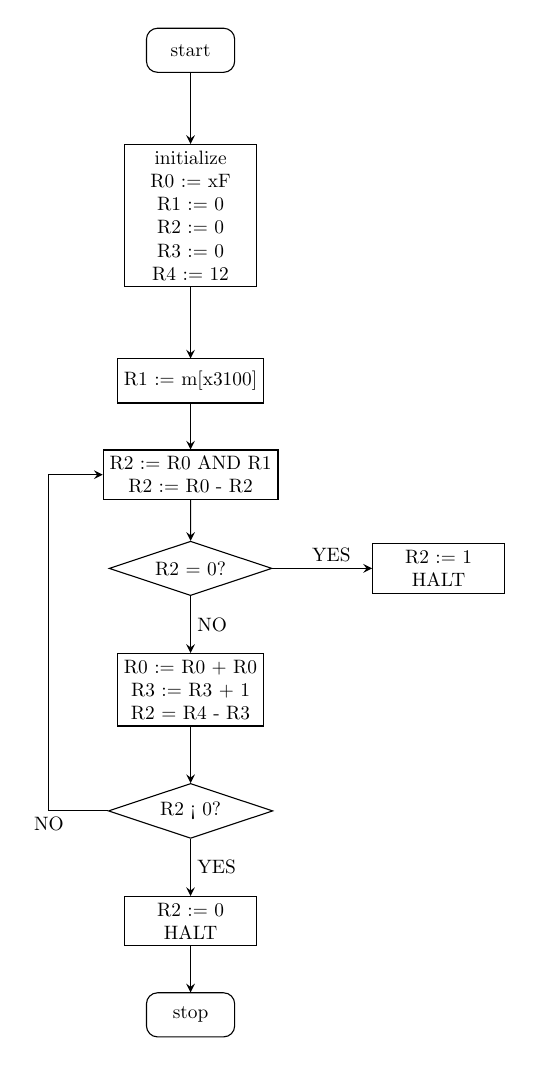
\begin{tikzpicture}[node distance=1.5cm, align=center]
  %定义流程图具体形状
  \node (start) [startstop] {start};
  \node (pro1) [process, below of=start, yshift= -1.5cm] {initialize \\ R0 := xF \\ R1 := 0 \\ R2 := 0 \\ R3 := 0 \\ R4 := 12};
  \node (pro2) [process, below of=pro1, yshift= -1.5cm] {R1 := m[x3100]};
  \node (pro3) [process, below of=pro2, yshift= -0.2cm] {R2 := R0 AND R1 \\ R2 := R0 - R2};
  \node (dec1) [decision, below of=pro3, yshift= -0.2cm] {R2 = 0?};
  \node (pro4) [process, right of=dec1, xshift = 3cm] {R2 := 1 \\ HALT};
  \node (pro5) [process, below of=dec1, yshift = -0.7cm] {R0 := R0 + R0 \\ R3 := R3 + 1 \\ R2 = R4 - R3};
  \node (dec2) [decision, below of=pro5, yshift= -0.7cm] {R2 < 0?};
  \node (pro6) [process, below of=dec2, yshift = -0.5cm] {R2 := 0 \\ HALT};
  \node (stop) [startstop, below of=pro6, yshift= -0.2cm] {stop};

  %连接具体形状
  \draw [arrow](start) -- (pro1);
  \draw [arrow](pro1) -- (pro2);
  \draw [arrow](pro2) -- (pro3);
  \draw [arrow](pro3) -- (dec1);
  \draw [arrow](dec1) -- ($(dec1.east) + (0.75,0)$) node[anchor=south] {YES} |- (pro4);
  \draw [arrow](dec1) -- node[anchor=west] {NO} (pro5);
  \draw [arrow](pro5) -- (dec2);
  \draw [arrow](dec2) -- ($(dec2.west) + (-0.75,0)$) node[anchor=north] {NO}|- (pro3);
  \draw [arrow](dec2) -- node[anchor=west] {YES} (pro6);
  \draw [arrow](pro6) -- (stop);
  \end{tikzpicture}
\caption{The flowchart of the program.}
\end{figure}

\section{Source code}
\linespread{0.9}      %行距缩小
\begin{Verbatim}[frame = single, numbers = left]
; .orig x3000
0011 0000 0000 0000

; initialize all register
0101 000 000 1 00000   ; R0 is ...1111...
0001 000 000 1 01111
0101 001 001 1 00000   ; R1 is the number to be tested
0101 010 010 1 00000   ; R2 is used to store tmp result
0101 011 011 1 00000   ; use R3 to count loop time
0101 100 100 1 00000   ; use R4 to store max loop time 12
0001 100 100 1 01100

0010 001 011111000     ; load the word into R1
0101 010 000 000 001   ; AND R2, R0, R1
1001 010 010 111111    ; R2 = R0 - R2
0001 010 010 1 00001
0001 010 010 000 000
; if R2 == 0, branch #7 and set R2 = 1 and HALT
0000 010 000000111
; else
0001 000 000 000 000   ; R0 <<= R0, left shift R0 for one bit
; count the loop time and determine stop loop or not
0001 011 011 1 00001   ; R3++
1001 010 011 111111    ; R2 = R4 - R3
0001 010 010 1 00001
0001 010 010 000 100
; if stop(R2 is negative), branch #3 and set R2 = 0 and HALT
0000 100 000000100
; if not stop, continue loop, branch #-12
0000 111 111110100

0101 010 010 1 00000   ; set R2 = 1 and HALT
0001 010 010 1 00001
1111 0000 0010 0101
0101 010 010 1 00000   ; set R2 = 0 and HALT
1111 0000 0010 0101
\end{Verbatim}
\linespread{0.9}      %行距恢复

\section{Questions TA asked you and your answer in check}
Question: Can you introduce your program?

Answer: First, I initialize the registers. I set R0 into \verb|0000 0000 0000 1111|, R1, R2, R3 into 0, and R4 into 12. I use R1 to store the number to be tested, use R2 to store tmp result, use R3 to count loop time, use R4 to store max loop time 12.

Then I load the word into R1.

Then, I store R0 AND R1 into R2. If now R2 - R0 = 0, it means there is a consecutive 4-bits of 1s, so I set R2 into 0 and stop the program. If R2 - R0 $\neq$ 0, it means there is no consecutive 4-bits of 1s so far, so I left shift R0 to test next 4 bits and add 1 to R3 to increase the loop time by 1.

Now I check whether I need to stop the loop. if R3 > R4, it means the loop needs to be terminated, so I terminiate the loop, set R2 into 0 and stop the program. If R3 $\leq$ R4, the loop continues, and the program goes back to the previous step.

\end{document}